\chapter{Исследование поведения метрик для различных типов графов} \label{chapt2}

\section{Генерация вершин графов} \label{sect2_1}

В данной работе вершины графа генерировались с помощью смеси гауссовских распределений. Основной случай:четыре двумерные гауссианы, центры которых расположены симметрично относительно начала координат, дисперсии и количество точек равны.

%по мере исследования добавить две гауссианы, равномерное распределение вершин, новые параметры.
%добавить графы от von Luxburg и многомерный случай

%\newpage
%============================================================================================================================


\section{Генерация невзвешенных графов} \label{sect2_2}

В данной работе рассматривались три класса случайных геометрических невзвешенных графов графов: 
\begin{enumerate}
  \item \textbf{$\varepsilon$-графы}: вершины соединяются ребром в том случае, когда евклидово расстояние между ними не превышает заданного параметра $\varepsilon$.
  \item \textbf{Симметричные графы ближайших соседей}: между двумя вершинами проводится ребро в том случае, если хотя бы одна из них попадает в множество $k$ ближайших соседей другой; параметр $k$ задан.
  \item \textbf{Mutual графы ближайших соседей}: две вершины соединяются ребром, если обе они попадают в множество $k$ ближайших соседей друг друга; параметр $k$ задан.
\end{enumerate}

Параметр графа ($\varepsilon$ или $k$) выбирался таким образом, чтобы граф оказался связным с высокой вероятностью. Это делалось потому, что наибольший интерес для машинного обучения представляют именно связные графы.

\begin{figure}[h]
  \begin{minipage}[h]{0.29\linewidth}
    \center{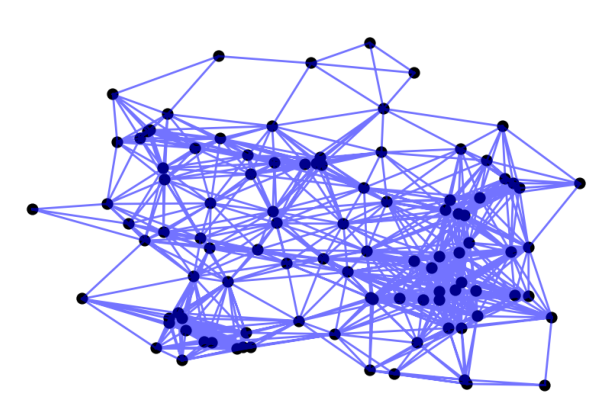
\includegraphics[width=0.95\linewidth]{epsilon} \\ а)}
  \end{minipage}
  \hfill
  \begin{minipage}[h]{0.29\linewidth}
    \center{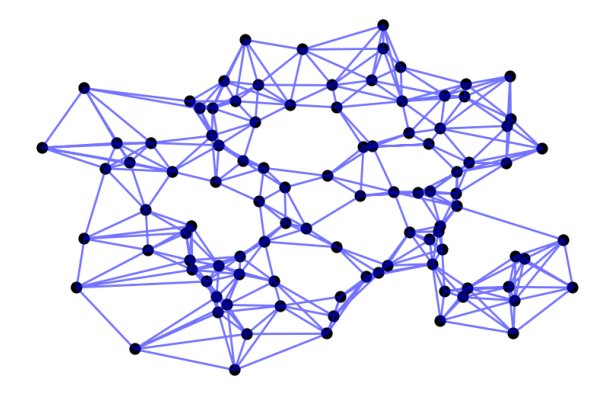
\includegraphics[width=0.95\linewidth]{sym_knn} \\ б)}
  \end{minipage}
  \hfill
  \begin{minipage}[h]{0.29\linewidth}
    \center{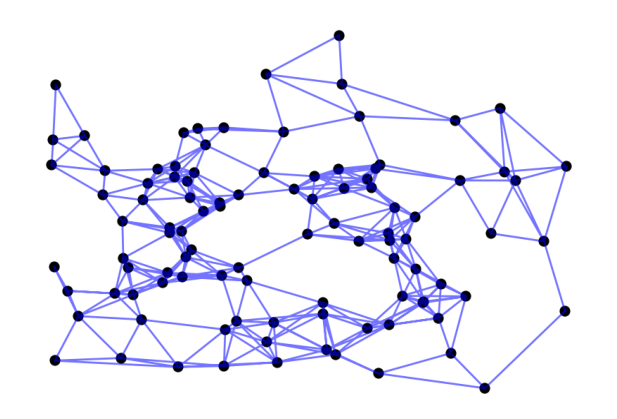
\includegraphics[width=0.95\linewidth]{mut_knn} \\ в)}
  \end{minipage}
  \caption{Примеры невзвешенных графов. Слева направо: $\varepsilon$-граф, симметричный граф ближайших соседей ($k=6$), mutual граф ближайших соседей ($k=9$).}
  \label{img:graphs}  
\end{figure}

%\newpage
%============================================================================================================================

\section{Генерация взвешенных графов} \label{sect2_3}

В данной работе взвешенные графы представлены гауссовскими графами. Это полные графы, в которых вес ребра между вершинами $i$ и $j$ определяется по формуле $w_{ij} = exp(-\frac{||v_i - v_j||^2} {\sigma^2} )$, где параметр $\sigma > 0$ задан.

%\newpage
%============================================================================================================================

\section{Сравнение метрик} \label{sect2_4}

Для каждого типа графов для различных значений параметра метрк вычислялись матрицы расстояний для каждой метрики, описанной в главе 1. Чтобы оценить <<качество>> метрик, они сравнивались с евклидовым расстоянием между вершинами графа. Для сравнения использовались коэффициент корреляции с евклидовым расстоянием и матричные нормы для матрицы $D_{euclid} - D_{metrics}$.


\clearpage
